\documentclass{article}
\usepackage{geometry}
\geometry{
	a4paper,
	%total={170mm,257mm},
	left=20mm,
	top=30mm,
}

\usepackage{fancyhdr}
\usepackage{tikz}
\usepackage{hyperref}
\usepackage{graphicx}
\usepackage{hyperref}
\usepackage{mdframed}
\usepackage{listings} % Include the listings package
\usepackage{xcolor}   % to define your own colors
\usepackage{subcaption}
\usepackage{array}

\bibliographystyle{unsrt}
\bibliography{references}


\newmdenv[
linecolor=blue, % Color of the border line
backgroundcolor=gray!20, % Background color; "gray!20" means "20% gray"
frametitle=Note, % Title of the frame, delete this line if you don't want a title
skipabove=\baselineskip, % Space above the frame
skipbelow=\baselineskip, % Space below the frame
]{mynote}

% code-snippets:
% Define the color styles you wish to use in the document for the Python syntax highlighting
\lstdefinestyle{mystyle}{
	backgroundcolor=\color{white},   % choose the background color; you must add \usepackage{color} or \usepackage{xcolor}
	commentstyle=\color{green},
	keywordstyle=\color{blue},
	numberstyle=\tiny\color{gray},
	stringstyle=\color{red},
	basicstyle=\ttfamily\footnotesize,
	breakatwhitespace=false,         
	breaklines=true,                 
	captionpos=b,                    
	keepspaces=true,                 
	numbers=left,                    
	numbersep=5pt,                  
	showspaces=false,                
	showstringspaces=false,
	showtabs=false,                  
	tabsize=2
}
\definecolor{LightGray}{gray}{0.9}

\lstset{style=mystyle} % Apply your style globally to the document


\newcommand{\LVA}{Reverse Engineering}
\newcommand{\LVAKURZ}{REV3}
\newcommand{\SEMESTER}{WS 2023/2024}
\newcommand{\UELABEL}{UE 05}
\newcommand{\UETITLE}{Firmware Analyse}
\newcommand{\AUTHOR}{Jakob Mayr}


\title{\vspace{5cm} \LVA\ (\LVAKURZ)\\ \vspace{1cm} \textbf{\UELABEL\ -- \UETITLE\ -- Protokoll} \vspace{2.5cm}}
\author{\AUTHOR}
\date{\SEMESTER}

\begin{document}
	
	\pagestyle{fancy}
	
	\maketitle
	
	\tikz [remember picture, overlay] %
	\node [shift={(3.7cm,-4cm)}] at (current page.north west) %
	[anchor=north west] %
	{
\includegraphics{fhooe_logo.jpg}};
	
	\tikz [remember picture, overlay] %
	\node [shift={(10cm,-4.8cm)}] at (current page.north west) %
	[anchor=north west] %
	{
\includegraphics{si_logo.jpg}};
	
	%\tikz [remember picture, overlay] %
	%\node [shift={(7.2cm,-11.65cm)}] at (current page.north west) %
	%[anchor=north west] %
	%{\includegraphics[scale=0.12]{./img/star_wars_logo_no_background.png}};
	%
	%\pagebreak
	
	\fancyhf{}
	\fancyhead[L]{\LVA\ (\LVAKURZ)}
	\fancyhead[C]{\UELABEL}
	\fancyhead[R]{\SEMESTER}
	\fancyfoot[L]{Seite \thepage\ von \pageref{LastPage}}
	\fancyfoot[R]{\AUTHOR}
	
	
	\pagebreak
	
	\section*{File-Beschaffung}
	Die benötigte Firmware-Version kann direkt auf der netgear-Seite heruntergeladen werden:\\
	\url{https://www.downloads.netgear.com/files/GDC/R6400/R6400-V1.0.1.12_1.0.11.zip}\\
	
	\section*{Analyse Teilkomponenten}
	Extrahieren des .zip-Archivs:\\
	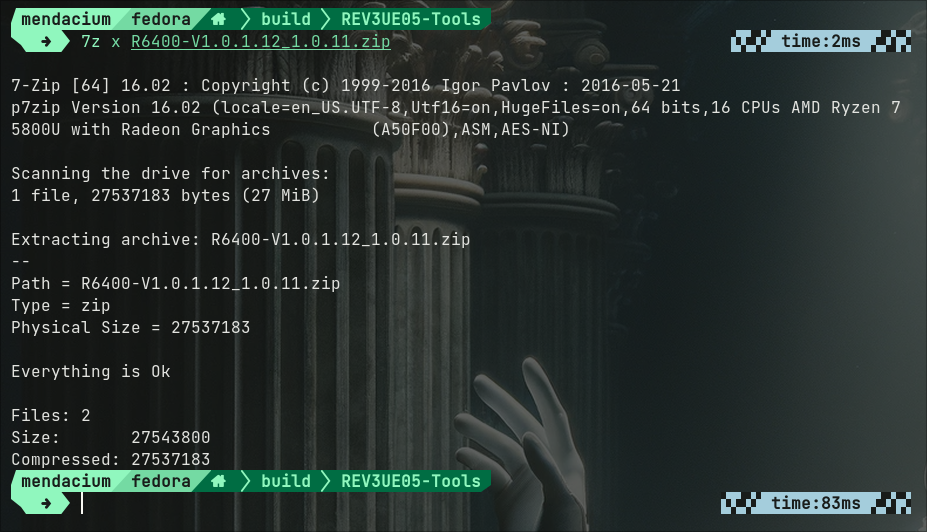
\includegraphics[width=0.5\linewidth]{"pictures/1.1 Extract.png"}\\
	Die Ausführung des Befehls \texttt{binwalk} mit der Option \texttt{--signature} auf die Datei \texttt{r6400-V1.0.1.12\_1.0.11.chk} liefert folgende Informationen über die Binärdatei der Firmware:\\
	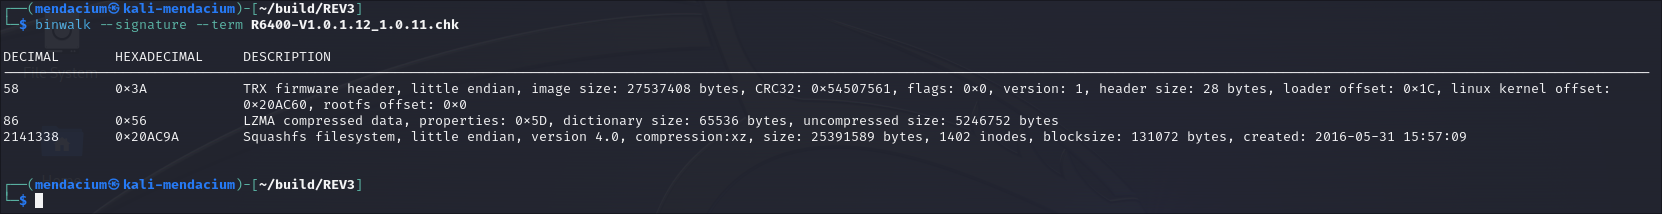
\includegraphics[width=1\linewidth]{"pictures/1.2 signature.png"}\\
	\begin{itemize}
		\item \textbf{TRX Firmware-Header:} Das Binärbild enthält einen TRX Firmware-Header, der häufig bei Firmware-Dateien für Router oder ähnliche Geräte verwendet wird. Er ist in Little-Endian-Format mit einer Größe des Images von 27.537.408 Bytes und enthält einen CRC32-Prüfsummenwert.
		
		\item \textbf{LZMA komprimierte Daten:} Der Teil der Datei enthält LZMA-komprimierte Daten. Dies schließt Eigenschaften, eine Wörterbuchgröße und die unkomprimierte Größe ein.
		
		\item \textbf{Squashfs-Dateisystem:} Das Binärbild umfasst ein Squashfs-Dateisystem. Squashfs ist ein komprimiertes, schreibgeschütztes Dateisystem für Linux. Die Version, der Kompressionstyp (xz), die Größe, die Anzahl der Inodes, die Blockgröße und das Erstellungsdatum werden ebenfalls angegeben.
	\end{itemize}
	Das Erstellungsdatum des Squashfs-Dateisystems ist der 31. Mai 2016 um 15:57:09 Uhr.\\
	
	\noindent\textbf{Extrahieren} der LZMA komprimierten Datei und des squashfs-Dateisystems:\\
	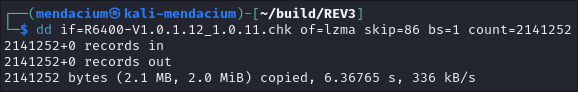
\includegraphics[width=0.4\linewidth]{"pictures/1.3 extract lzma.png"}\\
	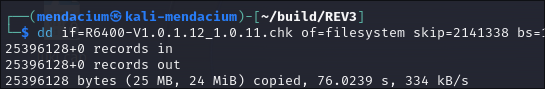
\includegraphics[width=0.4\linewidth]{"pictures/1.4 extract filesystem.png"}\\
	
	\pagebreak
	
	\noindent"\textbf{Mounten}" des Dateisystems in "\texttt{/mnt}":\\
	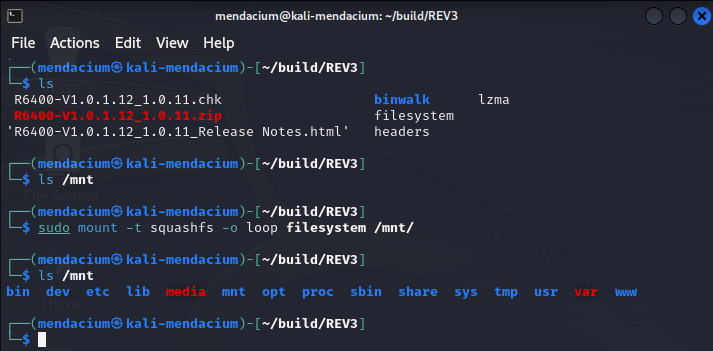
\includegraphics[width=0.4\linewidth]{"pictures/1.5 mount squashfs.png"}\\
	Suchen und finden der "httpd"-Binärdatei:\\
	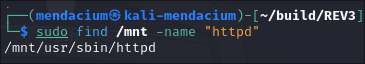
\includegraphics[width=0.4\linewidth]{"pictures/1.6 find httpd.png"}\\

	\subsection*{httpd}
	Informationen (radare2) über die Binärdatei:\\
	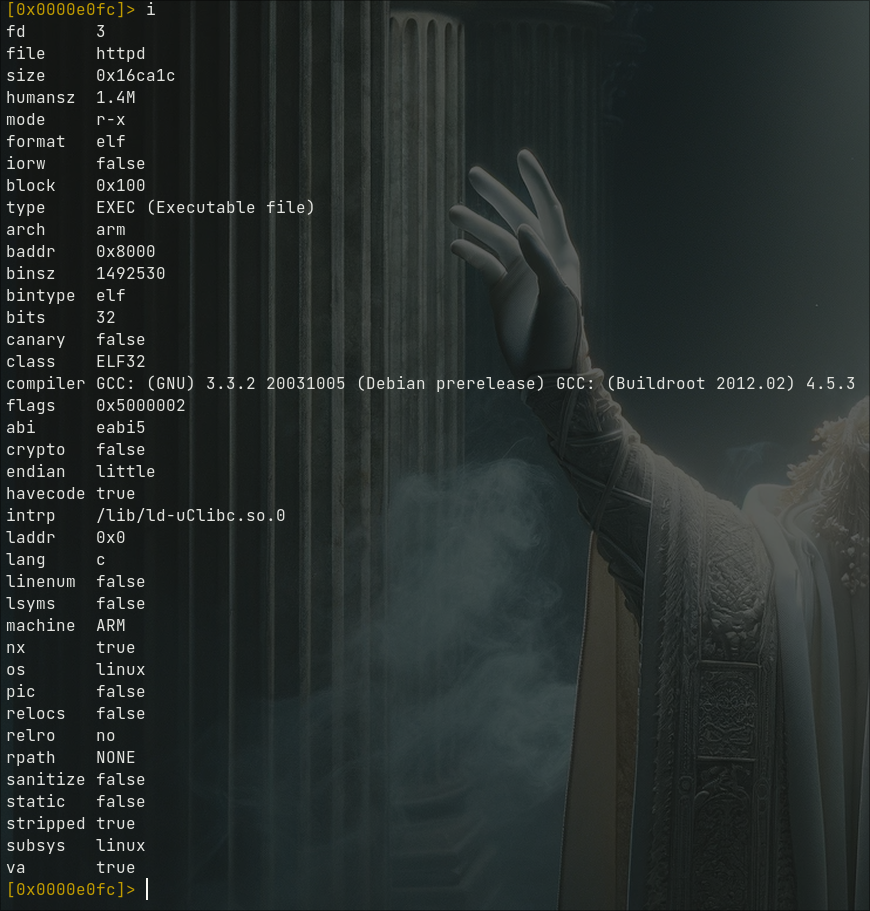
\includegraphics[width=0.4\linewidth]{"pictures/1.7 architecture, entry point.png"}\\
	
	\label{LastPage}
	
\end{document}